\section{Durchführung und Versuchsaufbau}


\noindent Die zentralen Bauteile für diesen Versuch sind eine Kupfer-Röntgenröhre und ein Geiger-Müller-Zählrohr.\\
Zwischen diese beiden Bauteile werden dann andere Bauteile wie ein LiF-Kristall, für die Bragg-Reflexion, oder ein Plexiglas-Streuer platziert.\\
Den experimentellen Aufbau inklusive des Zählrohrs, der Röntgenröhre und den anderen beschrifteten Bauteilen findet man in Abbildung \ref{img:aufbau}.



\begin{figure}[h]
    \centering
    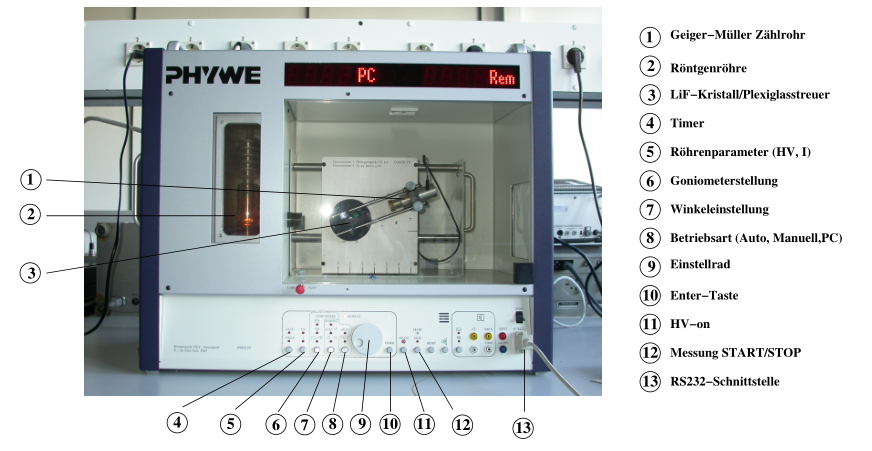
\includegraphics[width=0.75\textwidth]{latex/images/roentgenroehre.PNG}
    \caption{Der Aufbau der Messaparatur inklusiv Röntgenröhre\protect \cite{V603}.}
    \label{img:aufbau}
\end{figure}

\noindent
Für die Versuchsdurchführung wird an die Röntgenröhre eine konstante Beschleunigungsspannung von $\SI{35}{\kilo\volt}$ angelegt und ein Teilchenstrom von $\SI{1}{\milli\ampere}$ genutzt.\\\\
Zuerst soll das charakteristische Spektrum untersucht werden. Dafür wird eine $\SI{2}{\milli\metre}$ Blende vor der Röhre platziert und der LiF-Kristall in die drehbare Halterng gesteckt.\\
Damit werden nun die Beugungsmaxima erster Ordnung, alle 5 bis 10 Sekunden in $\SI{0.2}{\degree}$ Schritten, gemessen.\\



\begin{figure}[h]
    \centering
    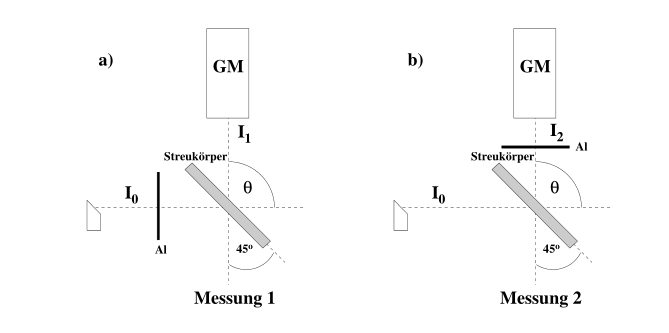
\includegraphics[width=0.70\textwidth]{latex/images/aufbau.PNG}
    \caption{Eine schematische Darstellung der Anordnung der verschiedenen Bauteile für die unterschiedlichen Messreihen\protect \cite{V603}.}
    \label{img:aufbau2}
\end{figure}

\noindent
Nun soll das Transmissionsverhalten des Aluminiumabsorbers untersucht werden. Dafür wird vor der Blende der Absorber installiert.
Für eine Messzeit von $\SI{100}{\second}$ kann damit nun die Intensität in Abhängigkeit des Winkels des Kristalls gemessen werden.\\
Diese Messung sollte einmal mit und einmal ohne Absorber durchgeführt werden um den Einfluss des Aluminiumabsorbers zu bestimmen.\\
Zusätzlich muss hier die Totzeit des Zählrohrs beachtet werden. Dafür kann die folgende Gleichung genutzt werden:
\begin{equation*}
    I = \dfrac{N}{1-\tau \cdot N}
\end{equation*}


\noindent
Für die nächste Messreihe wird eine $\SI{5}{\milli\metre}$ Blende genutzt und anstatt des LiF-Kristalls ein Plexiglas-Streuer.\\
Der Streuer soll dabei auf $\SI{45}{\degree}$ und das Zählrohr auf $\SI{90}{\degree}$ eingestellt werden.
Damit soll nun die Intensität $I_0$ der Röhre gemessen werden.\\
In der Abbildung \ref{img:aufbau2} ist dieser Aufbau schematisch noch einmal schematisch dargestellt.\\\\

\noindent
Im Folgenden soll nun wie in Abbildung \ref{img:aufbau2} dargestellt, der Aluminiumabsorber einmal in 
den Strahlengang zwischen Röntgenröhre und Streukörper und einmal in den Strahlengang
zwischen Streukörper und Zählrohr gebracht werden.
Damit können dann die Transmissionen $T_1=\frac{I_1}{I_0}$ und $T_2=\frac{I_2}{I_0}$, welche mit den gestreuten und ungestreuten Wellenlängen korrespondieren, bestimmt werden.\\
Diese Messungen sollen fünf mal durchgeführt werden.

